\documentclass[12pt]{article}%
\usepackage{amsfonts}
\usepackage{amsmath}
\usepackage[a4paper, top=2.5cm, bottom=2.5cm, left=2.2cm, right=2.2cm]%
{geometry}
\usepackage{times}
\usepackage{amsmath}
\usepackage{amssymb}
\usepackage{mathtools}
\DeclarePairedDelimiter\ceil{\lceil}{\rceil}
\DeclarePairedDelimiter\floor{\lfloor}{\rfloor}
\newenvironment{proof}[1][Proof]{\textbf{#1.} }{\ \rule{0.5em}{0.5em}}

\begin{document}

\title{CS 590 HW 1}
\author{Edward Kim}
\date{\today}
\maketitle

\section{Problem 1 (c)}
\begin{proof}
  Let $f$ be an $n$-ary Boolean function with $\mathcal{L}(f)$ denoting its leafsize. Define the following map $\mu:\{n \text{-ary Boolean functions}\} \rightarrow \mathbb{R}_{\geq 0}$. Given a Demorgan formula $F$ for function $f$, let $V_F$ denote the set of variables used as inputs in $F$. Define $\mu(f) = \min_{F} |V_F|$ taken over all formulae $F$ computing function $f$. We claim that this is a formal complexity measure in accordance to the definition, and check the relevant criteria:
  \begin{enumerate}
    \item If $f$ is a constant function i.e $ f = 0, 1$, then $f$ does not depend on any variable input. Thus, $\mu(f) = 0$.
    \item If is a coordinate function, $f$ only depends on the relevant coordinate variable. For the coordinate function $f(x) = x_i$ The formula will simply be an input variable $x_i$ acting as the output as well.
    \item For the conjunction of two formulas $f \wedge g$, observe that if $\mu(f)$ and $\mu(g)$ are the minimal number of variables required to compute $f,g$ respectively, then new formula $f \wedge g$ does not require more than $\mu(f) + \mu(g)$ new variables. This bound is saturated when the corresponding sets of variables used to compute $f,g$ are disjoint. We arrive at $\mu(f \wedge g) \leq \mu(f) + \mu(g)$. The analysis for $\mu(f \vee g) \leq \mu(f) + \mu(g)$.
  \end{enumerate}
  %
  Using our definition of $\mu$, it immediately follows that $\mu(AND_n) \geq n$. Indeed, no formula computing $AND_n$ can depend on fewer than all $n$ inputs. Combining this with our third property above, we conclude that $\mu(AND_n) = n$.
\end{proof}

\section{Problem 2}
\begin{enumerate}
  \item
  \begin{proof}
    We prove our lower bound through an induction argument. The case when $n=1$ is simple to check as there are at least $2$ monotone $1$-ary Boolean functions (just take the two constant functions $f = 0,1$). Now assume the hypothesis for $n-1$-ary Boolean functions and consider the case for the set of $n$-ary Boolean functions.
    %
    Let $x,y \in \{0,1\}^{n-1}$ denote two $n-1$ bit strings, and let $x\cdot \{0,1\}$ denote the string $x$ with $0,1$ appended to the right-end of $x$. Naturally extend this definition to strings $y\cdot \{0,1\}$.  We deduce the following inequalities assuming that $x \leq y$:
    $$ x \cdot 0 \leq y \cdot 0, \; x \cdot 1 \leq y \cdot 1, \; x \cdot 0 \leq y \cdot 1 $$
    It follows we can induce a monotone $n$-ary Boolean function from an $n-1$-ary Boolean function, by simply setting the $x\cdot 1 \mapsto f(x)$ for $x \in \{0,1\}^{n-1}$ to be a monotone Boolean function and fixing the $x \cdot 0 \mapsto 0$. This gives us an immediate $2^{n-1 \choose \floor{\frac{n-1}{2}}}$ monotone $n$-ary Boolean functions through the induction hypothesis. In fact, by being careful with our bookkeeping, we can find another 15 monotone $n$-ary Boolean functions where lower $x \cdot 0$ and upper $x \cdot 1$ elements do not have to all map to $0,1$ respectively.
    %
    Furthermore, observe that this extends to any $n-1$ subset of indices $[n]$. In other words, let $\mathcal{C}_{i,0}(x) = x_1 \cdot x_2 \cdots x_{i-1} \cdot 0 \cdot x_{i} \cdots x_{n-1} $ be the string $x$ with $0$ placed in the $i^{th}$ index. We can repeat the same scheme above:
    $$ \mathcal{C}_{i,1}(x) \mapsto f(x), \; \mathcal{C}_{i,0}(x) \mapsto 0 \quad x \in \{0,1\}^{n-1}$$

    These give us different sets of monotone Boolean functions since the $\mathcal{C}_{i,0}, \mathcal{C}_{i,1}$ partitions the set of all $n$ bit srings $\{0,1\}^n$ differently for each $i \in [n-1]$.

    This gives us $n$ distinct $2^{n-1 \choose \floor{\frac{n-1}{2}}}$ sets of monotone $n$-ary Boolean functions. Now notice that
    %
    $$ \frac{n}{(n/2)^2}{n-1 \choose \floor{\frac{n-1}{2}}} \geq {n \choose \floor{\frac{n}{2}}}$$
    So, $16n2^{{n-1 \choose \floor{\frac{n-1}{2}}}} = 2^{4\log n {n-1 \choose \floor{\frac{n-1}{2}}}} \geq 2^{\frac{4}{n} {n-1 \choose \floor{\frac{n-1}{2}}}} \geq 2^{{n \choose \floor{\frac{n}{2}}}}$, giving us the desired result.
    \end{proof}
    %
    \item
    \begin{proof}
      We calculate the following probability of a montone $n$-ary Boolean function having circuit size less than $2^n/n^{1.5}$: Let $M_n$ denote the set of all $n$-ary monotone Boolean functions.
      \begin{gather*}
        \mathbb{P}_{f \sim M_n} [ \mathcal{C}(f) \leq 2^n/n^{1.5}] = \frac{|\{\text{$n$-ary monotone functions with $\mathcal{C}(f) \leq 2^n/n^{1.5}$}\}|}{|M_n|} \leq \\
        \frac{|\{\text{$n$-ary Boolean functions with $\mathcal{C}(f) \leq 2^n/n^{1.5}$}\}|}{|M_n|} \leq \frac{(2^n/n^{1.5})^{2^n/n^{1.5}}}{2^{\Omega(2^n/n^{1.5})}} = \\
        \frac{2^{n2^n/n^{1.5}}}
        {n^{1.5 \cdot 2^n / \sqrt{n}}2^{\Omega(2^n/\sqrt{n})}} =
        \frac{ 2^{ 2^n/\sqrt{n} - \Omega(2^n/\sqrt{n})} }
             {n^{1.5 \cdot 2^n/\sqrt{n}}} = \frac{1}{{n^{\frac{1.5 \cdot \Omega(1)\cdot2^n}{\sqrt{n}} }} } = o(1)
      \end{gather*}
      Thus,
      $\mathbb{P}_{f \sim M_n} [ \mathcal{C}(f) > 2^n/n^{1.5}] = 1 - o(1) $ as required.
    \end{proof}
  %
\end{enumerate}

\section{Problem 3 (c)}
\begin{proof}
  Let $F$ be a minimal DeMorgan formula computing $f$ with $\mathcal{L}(f)$ leafsize. We can simply compute the dual by
  \begin{enumerate}
     \item Adding negation gates to the beginning of each input variable in the formula.
     \item Adding a negation gate before the output variable of $F$
  \end{enumerate}
  Note that this does not change the formula leafsize. Thus, $\mathcal{L}(f) \geq \mathcal{L}(f^{\dagger})$. However, through direct calculation, it is simple to show that $(f^{\dagger})^{\dagger} = f$. By repeating the same argument above on $f^{\dagger}$, we yield that $\mathcal{L}(f^{\dagger}) \geq \mathcal{L}((f^{\dagger})^{\dagger})$. This implies that $\mathcal{L}(f^{\dagger}) \geq \mathcal{L}(f)$, showing that $\mathcal{L}(f^{\dagger}) = \mathcal{L}(f)$.
\end{proof}

\section{Problem 5}
\begin{enumerate}
  \item
  \begin{proof}
  To show the lower bound, define the following partitioning scheme on the $\ceil{2^k/k} \times k \approx 2^k$ input bits of $\bf{Andreev}_{k,m}$.
  \begin{enumerate}
    \item Define the first partition $V_1$ to be the first $2^k$ bits. This will the partition containing the truth table of the $k$-ary input function
    \item Define the partitions $V_{i+1}, \; 0 \leq i \leq \ceil{2^k/k} = m$ to be the set of indices $$ V_{i+1} = \{\ell \cdot \ceil{2^k/k} + i \}_{0\leq \ell \leq k-1}$$ In other words, the $i^{th}$ index for each copy of $XOR_m$ present in $\bf{Andreev}_{k,m}$.
  \end{enumerate}
  We can now bound the number of subfunctions. For $\text{sub}_{V_1}({\bf Andreev}_{k,m})$, it follows from the definition of ${\bf Andreev}_{k,m}$ that every subfunction is of the form:
  $$ f \mapsto f(h_1,...,h_k) $$ where the $h_1,...,h_k$ are constants induced from restriction $\rho$ assigning constants $\{0,1\}$ to the $km$ input variables. This function splits the set of all $n$-ary Boolean functions in half, namely the two sets:
  \begin{gather*}
    F_0(h_1,...,h_k) = \{f \mid f(h_1,...,h_k) = 0\} \\
    F_1(h_1,...,h_k) = \{f \mid f(h_1,...,h_k) = 1\}
  \end{gather*}
  Consequently, each string $h_1,...,h_k$ will induce different sets $F_0(h_1,...,h_k)$ and $F_1(h_1,...,h_k)$, which further induces different subfunctions. Thus, we have the bound:
  $$|\text{sub}_{V_1}({\bf Andreev}_{k,m})| \geq 2^k $$
  For the parititons $V_{i+1}$, observe that every restriction sets the truth table of a particular $k$-ary function in the first $2^k$ bits and sets the value for $XOR_{m-1}$ for the $k(m - 1)$ remaining input bits lying outside of $V_{i+1}$. Consequently, we at least have functions of the form:
  $$ y_1,...,y_m \mapsto \tilde{f}(y_1,...,y_m) $$ for all $\tilde{f}$ $n$-ary Boolean functions. This directly shows that
  $|\text{sub}_{V_1}({\bf Andreev}_{k,m})| \geq 2^{2^k}$.
  Finally, we invoke the Nechiporuk bound:
  \begin{gather*}
  \begin{split}
      \mathcal{L}_{B_2}({\bf Andreev}_{k,m}) & \geq  \frac{1}{4} \sum_{i=1}^{2^k/k} \log |\text{sub}_{V_i}(f)| + \frac{1}{4}\log |\text{sub}_{V_1}(f)| \\
      & \geq \frac{1}{4} \sum_{i=1}^{2^k/k} \log 2^{2^k} + \frac{1}{4}\log 2^k
      =  \frac{2^k2^k}{4k} + \frac{k}{4} = \Omega(n^2/\log n)
  \end{split}
  \end{gather*}
\end{proof}
%
\item
\begin{proof}
  I only give a partial solution to this exercise, namely the naive $O(2^kkm)$ bound. This bound is achieved by explicitly constructing the following $B_2$ formula roughly shown in Figure \ref{fig:cir1}.

  \begin{figure}
    \centering
    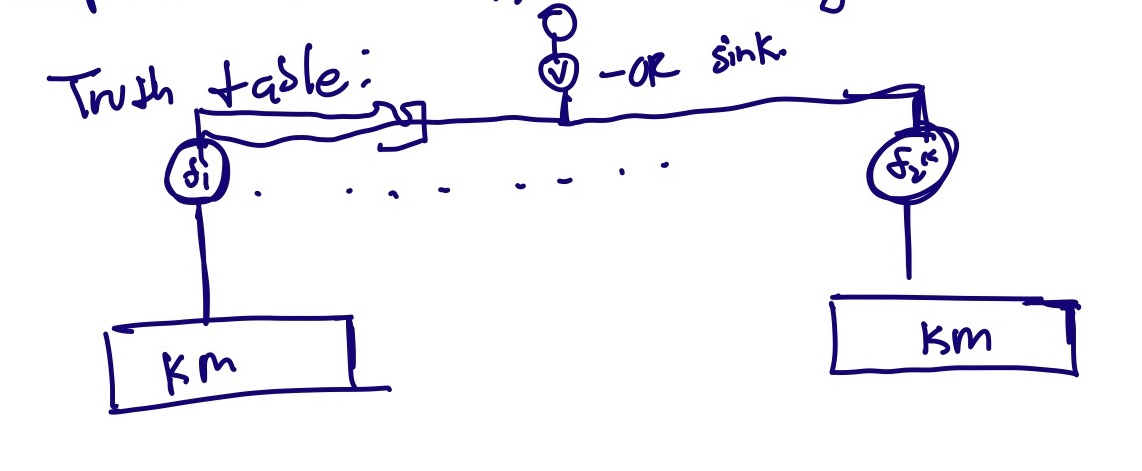
\includegraphics[width=10cm, height=4cm]{./Page4.jpeg}
    \caption{Rough drawing of $B_2$ formula}
    \label{fig:cir1}
  \end{figure}
  The formula first computes all $k$ $XOR_m$ values in tandem. Then the computed values are checked against all $2^k$ truth-table values. If equality holds, then the formula passes the corresponding truth-table value along. Otherwise, it passes zero. All $2^k$ values are passed then into an $OR$-sink which outputs the correct value of ${\bf Andreev}_{k,m}$. This gives the naive $O(2^k km)$ lower bound.
\end{proof}

\end{enumerate}

\section{Problem 6}
\begin{proof}
  Let $f: \{0,1\}^n \rightarrow \{0,1\}$ be some $n$-ary Boolean function. We calculate the bounds for $|\text{sub}_{V_i}(f)|$ if we divide partition our index set $[n]$ into disjoint sets of size $\log n$. First, assume that $n/\log n$ is an integer. For partitions of size $\log n$, we have that:
  $$ |\text{sub}_{V_i}(f)| \leq 2^{2^{\log n}} = 2^n $$
  Combining this observation with the Nechiporuk form, we yield that:
  $$ \frac{1}{4} \sum_{i=1}^k \log |\text{sub}_{V_i}(f)| \leq \frac{1}{4} \sum_{i=1}^{n/\log n} \log 2^n = O(n^2/\log n) $$
  We can then extend to the case where  $n / \log n$ may not be an integer i.e there exists a partition with size stricter smaller than $\log n$. Let $V_p$ be such a partition and assume that it is at the end of $[n]$. Then we know that $\log |\text{sub}_{V_p}(f)| < n$. We compute the Nechiporuk form once more:
  $$ \frac{1}{4} \sum_{i=1}^k \log |\text{sub}_{V_i}(f)| \leq \frac{1}{4}\sum_{i =1}^{O(n/\log n)} \log 2^n  = O(n^2/\log n)$$
  as required.
\end{proof}

\section{Problem 7}
\begin{enumerate}
  \item
  \begin{proof}
    We can create such a constant depth circuit by implementing a basic adder with carry-over. Consider the simple case for one-bit addition between two bits $x,y \in \{0,1\}$:
    \begin{enumerate}
      \item Output $u_1$ will be $x \oplus y$, so it suffices to designate the carryover rules for the second bit $u_2$. Let $c = x \wedge y$ be the carryover bit.
      \item $u_2 = 1$ iff one of the following cases hold:
      %
      \begin{align*}
          x = 0, \; y =1,\; c = 1 \\
          x = 1, \; y = 0,\; c = 1 \\
          x = 1, \;y = 0,\; c = 0,1
      \end{align*}
      These cases can be decided using a constant depth circuits.
    \end{enumerate}
    Observe that such a circuit can easily be extended to an arbitrary number of bits inductively without increasing depth. This is achieved by duplicating the machinery in part (a) and appended another parity gate to account for the carryover bits. For instance, we can extend the one bit gate above to two-bits by adding the circuit $u_2 = c_1 \oplus (x_2 \oplus y_2)$ where $c_1 = x_1 \wedge x_2$. Finally, we calculate $c_2 = x_2 \wedge y_2$ for computation outlined in part (b).

    In addition, for $n$-bit numbers $x,y,z$, we can simply output $x+y$ through the adder and separately output $z$ as an $n+1$-bit number by prefixing $z$ with 0.
  \end{proof}
  %
  \item
  \begin{proof}
    Recall that the Hamming weight of an $n$ bit-string $x$ is $|x| = \sum
    _{i=1}^nx_i$. We will leverage the circuit created above to add the $x_i$ as a sequence of one-bit numbers. First, divide our input variables into $n/3$ disjoint partitions of $[n]$. If $n/3$ is not an integer, add the necessary number of dummy constants equating to zero. Run the adder circuit above on each of these paritions to create $2n/3$ new output nodes corresponding to the two-bit numbers storing the sum for each paritition. Repeat the same scheme again. Divide the set of two-bit numbers into partitions of three with $2n/9$ parititions in all. After adding the required dummy constants, apply the two-bit adder circuit to each of the partitions. We see that for eiteration $n$ of the construction, a linear factor of the total number of $n-1$ bit numbers remaining is removed by the adder circuit. Thus, this iteration can only occur $\log n$ times. Addressing the bloating of the set through dummy constants, we see that the circuit has to add at most two more dummy constants at each iteration, meaning this routine adds at most $2\log n$ to the circuit size. Since the adder circuit only requires constant depth, the total depth of the circuit is at most $c \log n$ for some constant $c$.
  \end{proof}
  %
  \item
  \begin{proof}
    Let $C(x_1,...,x_n)$ be the circuit above which outputs a $n+1$ bit number storing the Hamming weight $|x|$. Since the output of a symmetric function $f$ only depends on $|x|$, we can hardcode our conditions into the circuit as follows:
    \begin{enumerate}
       \item Test equality between $|x|$ and all $\log n$ bit-sting $y, \; 0 \leq y \leq 2^{\log n} = n$ in tandem by testing equality one bit at a time for each $y$. This only requires constant depth and $O(n)$ size circuits to accomplish. This gives us the means to hardcode the output case-by-case.
       \item For each of the $n$-cases, hardcode the correct output in accordance to $f$. For instance, in $MAJ_n$, all cases where $|x| < n/2$ will output zero and all cases where $|x| > n/2$ will equal one. This only requires constant number of gates to accomplish.
    \end{enumerate}
    Thus, if we add all of the involved component circuits, we yield a $O(n)$ size and $O(\log n)$ depth DeMorgan circuit computing $f$. Since $f$ was chosen to be arbitrary, we conclude that all symmetric functions can be computed through such circuits.
  \end{proof}
\end{enumerate}


\end{document}
